% \section{General inverter concepts}
% \label{inverter}

% In the presented project an inverter from SMA with model number STP20000 of the Pulse Width Modulation(PWM)-type was provided. This kind of unit is capable of creating both active- and reactive-power from 3-phase voltages and currents in accordance with the load on the system. Although the control for such electronic devices can vary in a wide range, there are existing several schemes to generate AC voltage from DC via PWM. Out of several techniques, a scheme called sinusoidal pulse width modulation (SPWM) is assumed and will be discussed, as the outcome of applying other schemes will be somewhat similar and the SPWM scheme provides a basic understanding of the working principle.

% Despite the fact that the project deals with a 3-phase inverter, it is sufficient to introduce the basic concepts of operation in a 1-phase example.
% A basic hardware structure allowing for PWM control is a H-bridge as seen on \figref{fig:inverterblock}, more advanced and sophisticated structures are most likely used in the provided inverter as these improve both efficiency, noise canceling and leakage currents, but the working principle is somewhat the same \cite{aau_invert_topologies}. 


% \begin{figure}[H]
% \centering
% \begin{circuitikz}[thin,scale=1, every node/.style={scale=0.78}]

% % TRANSISTORS
% \draw
% (0,2) node[nigfete] (t1) {}
% (0,0) node[nigfete] (t2) {}
% (2,2) node[nigfete] (t3) {}
% (2,0) node[nigfete] (t4) {};
% \draw
% (t1.S) to[short] (t2.D)
% (t3.S) to[short] (t4.D);
% % DIODES and transistor labels
% \foreach \num in {1,2,3,4} {
% \node[anchor=south] at (t\num.G) {$T_\num$};
% \draw (t\num.S)++(0,0.5) -- ++(0.3,0) to[sD*] ($(t\num.D)+(0.3,-0.5)$) -- ++(-0.3,0);
% }          
% % BATTERY connection
% \draw
% (t4.S) to[short,-*] (t2.S) to[short] ($(t2.S)+(-2,0)$)
% to[battery,l=$U$] ($(t1.D)+(-2,0)$) to[short,-*] (t1.D) to[short] (t3.D);
% % RL
% \draw
% (t1.S) to[short,*-] ($(t1.S)+(3,0)$) to[short] ($(t1.D)+(3,0)$) coordinate (p1)
% to[R,l_=$R$] ++(2,0) to[L,l_=$L$,i>^=$i_L$] ++(3,0) coordinate (p);
% \draw
% (t4.D) to[short,*-] ($(t4.D)+(1,0)$) to[short] ($(t4.S)+(1,0)$) coordinate (n1)
% to[short] ++(5,0) coordinate (n);
% % C
% \draw
% (p) to[C,l=$C$,i>^=$i_C$,v<=$U_C$] (n);
% % LOAD
% \draw
% (p) to[short,*-]($(p)+(2,0)$) to[R,l=$LOAD$,i>^=$i_o$] ($(n)+(2,0)$) to[short,-*] (n);
% % U_i
% \draw
% (p1) to[open,v^=$U_i$] (n1);

% \end{circuitikz}
% \caption{Full-bridge inverter with load}
% \label{fig:inverterblock} 
% \end{figure}

% Most of the inverters usually deal with a full-bridge topology consisting of MOSFETs or IGBTs. The 1-phase circuit illustrated in \figref{fig:inverterblock} has four semiconductor switches with protection diodes, making it possible to create both current and voltage signals with controllable magnitude and frequency, thus controllable active and reactive power components. Each of these switches are controlled by the modulated control signal, namely $T_1$ and $T_4$ with $S$ while $T_2$ and $T_3$ with  $\neg{S}$ which is the negated signal of $S$.

% The scheme of modulating $S$ can be seen in \figref{fig:sinPWM} where a sine (control signal - $V_{control}$) and a triangular (reference signal - $V_{tri}$) are compared.   

% \begin{figure}[H]
% \centering
% 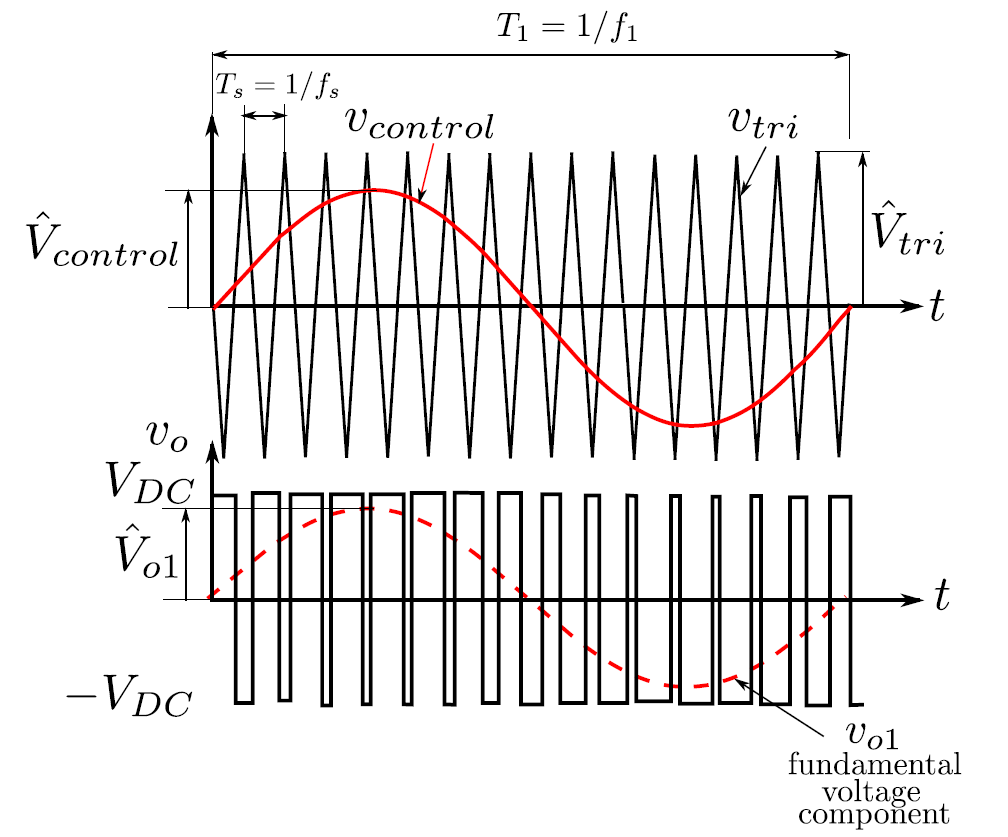
\includegraphics[width=0.6\textwidth]{rapport/analyse/sinPWM}
% \caption{Sinusoidal PWM \cite{bud_inverter_PV}}
% \label{fig:sinPWM}
% \end{figure}

% As can be seen, there are two cases given. When 
% \begin{equation} 
% \label{eq:case1}
% V_{control} > V_{tri} %\unit{W}
% \end{equation}
% then $T_1$ and $T_4$ are conducting, thus switching the DC voltage coming from the PV, while $T_2$ and $T_3$ are turned off. However, when 
% \begin{equation} 
% \label{eq:case1}
% V_{control} < V_{tri}
% \end{equation}
% then $T_2$ and $T_3$ are conducting and switching $V_{DC}$ therefore $T_1$ and $T_4$ are turned off. As can be seen, this switching pattern results in a PWM output signal with a sinusoidally varying duty cycle. While the output voltage is a square signal, the output current can result in an almost perfectly sinus wave(according to the load on the system) if the switching frequency is sufficiently high. Thus, as mentioned previously usually an LC or LCL filter is applied to the inverter voltage output in order to dampen the high frequency components. 

% The frequency of the desired output voltage can be determined by the frequency of the control signal $f_1$ which is the fundamental component of the waveform. The switching frequency equals to the frequency of $V_{tri}$, while the magnitude of the triangular waveform is usually kept constant in order to simplify the control of the voltage and frequency. Therefore the two modulation indexes can be given as: 
% \begin{equation} 
% \label{eq:ma}
% m_a = \frac{\tilde{V}_{control}}{\tilde{V}_{tri}}
% \end{equation}
% \begin{equation} 
% \label{eq:mf}
% m_f = \frac{f_1}{f_s}
% \end{equation}

% where $\tilde{V}_{control}$ and $\tilde{V}_{tri}$ are magnitudes of the signals.

% As can be seen from the relations, the controller of the inverter should measure frequency and voltage of the output waveforms at the same time to modify $m_a$ and to align the desired frequency by adjusting $m_f$.






